\documentclass{standalone}
\usepackage{tikz}
\usetikzlibrary{3d,arrows, calc, backgrounds, petri, positioning, shadows, shapes}


\tikzset{
	persp/.style={scale=3.0,x={(-0.8cm,-0.4cm)},y={(0.8cm,-0.4cm)}, z={(0cm,1cm)}},
	points/.style={fill=white,draw=black,thick}
	grid/.style={very thin,gray},
	axis/.style={->,ultra thick},
	cube/.style={thick, fill=black!15,opacity=0.5},
	cube hidden/.style={dashed},
	block/.style={
		rectangle, rounded corners,
		draw=black!80,
		fill=black!10, fill opacity=0.5,
		text=black!90, text opacity=1.0,
    text height=1.5ex,
    text depth=.25ex,
    text width=6em,
    text centered
	}
}

\tikzstyle{class}			=[rectangle, rounded corners, draw=black, fill=blue!40, drop shadow, text centered, anchor=north, text=white,    text width=3cm]
\tikzstyle{module}		=[rectangle, rounded corners, draw=black, fill=red!40, 	drop shadow, text centered, anchor=north, text=white,    text width=3cm]
\tikzstyle{component}	=[rectangle, rounded corners, draw=black, fill=green,   drop shadow, text centered, anchor=north, text=black!90, text width=3cm]
\tikzstyle{single}		=[text height=1.5ex, text depth=0.25ex]
\tikzstyle{double}		=[text height=4.0ex, text depth=2.75ex]
\tikzstyle{triple}		=[text height=6.5ex, text depth=5.25ex]
\tikzstyle{quadru}		=[text height=9.0ex, text depth=7.75ex]
\newcommand*{\rootPath}{../}

\begin{document}
\begin{tikzpicture}[persp]

	\def\i{10}
	\pgfmathparse{cos(\i)}\let\ci\pgfmathresult
	\pgfmathparse{sin(\i)}\let\si\pgfmathresult	
	\def\t{5}
	\pgfmathparse{cos(\t)}\let\ct\pgfmathresult
	\pgfmathparse{sin(\t)}\let\st\pgfmathresult
	\def\p{60}
	\pgfmathparse{cos(\p)}\let\cp\pgfmathresult
	\pgfmathparse{sin(\p)}\let\sp\pgfmathresult

	\def\sc{.5}
		
	\coordinate	(Ocube)	at (0,0,0);
	\coordinate	(Xcube)	at (\ci,\si,0);
	\coordinate	(Ycube)	at (-\si,\ci,0);
	\coordinate	(Zcube)	at (0,0,1);

	\coordinate	(Ocamera)	at ($(Ocube)-6*(Xcube)-5*(Ycube)-2*(Zcube)$);
	\coordinate	(Xcamera)	at (\ct*\cp,\ct*\sp,\st);
	\coordinate	(Ycamera)	at (-\sp,\cp,0);
	\coordinate	(Zcamera)	at (\st*\cp,\st*\sp,\ct);
	






	\def\scale{6}
	\foreach \t in {0,15,...,180}
	{
		\draw[black!50] ($(Ocube)+\scale*({cos(\t)},0,{sin(\t)})$)
		\foreach \rho in {5,10,...,355}
			{--($(Ocube)+\scale*({cos(\t)*cos(\rho)},{cos(\t)*sin(\rho)},{sin(\t)})$)}--cycle;
	}	
	\foreach \t in {135,150,...,315}
	{
		\draw[black!50] ($(Ocube)+\scale*({cos(\t)},{sin(\t)},0)$)
		\foreach \rho in {5,10,...,90}
			{--($(Ocube)+\scale*({cos(\t)*cos(\rho)},{sin(\t)*cos(\rho)},{sin(\rho)})$)};
	}
	% \foreach \t in {0,15,...,360} \draw[black!50] (Ocube)--($(Ocube)+\scale*({cos(\t)},{sin(\t)},{0})$);





	\node[yslant=+0.13,anchor=center,opacity=1]  at ($(Ocamera)-3*(Xcamera)$){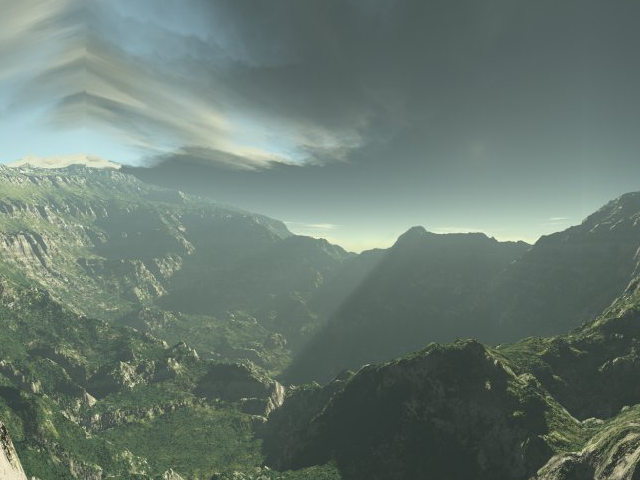
\includegraphics[width=11.8cm,height=6.8cm]{\rootPath Imgs/cubemap_fragment.png}};

	\coordinate (SVV0) at ($(Ocamera)-3*(Xcamera)+1.8*(Ycamera)+1.2*(Zcamera)$);	
	\coordinate (SVV1) at ($(Ocamera)-3*(Xcamera)+1.8*(Ycamera)-1.2*(Zcamera)$);	
	\coordinate (SVV2) at ($(Ocamera)-3*(Xcamera)-1.8*(Ycamera)+1.2*(Zcamera)$);	
	\coordinate (SVV3) at ($(Ocamera)-3*(Xcamera)-1.8*(Ycamera)-1.2*(Zcamera)$);	
	\draw[dashed, ultra thick, red] (SVV0)--(SVV1)--(SVV3)--(SVV2)--cycle;
	\draw[dashed, ultra thick, red] (Ocamera)--(SVV0);
	\draw[dashed, ultra thick, red] (Ocamera)--(SVV1);
	\draw[dashed, ultra thick, red] (Ocamera)--(SVV2);
	\draw[dashed, ultra thick, red] (Ocamera)--(SVV3);


	%%   S M A R T P H O N E
	\coordinate (S0) at ($(Ocamera)-.2*(Xcamera)-1.2*(Ycamera)-2.0*(Zcamera)$);
	\coordinate (S1) at ($(Ocamera)+.0*(Xcamera)-1.2*(Ycamera)-2.0*(Zcamera)$);
	\coordinate (S2) at ($(Ocamera)-.2*(Xcamera)+0.4*(Ycamera)-2.0*(Zcamera)$);
	\coordinate (S3) at ($(Ocamera)+.0*(Xcamera)+0.4*(Ycamera)-2.0*(Zcamera)$);
	\coordinate (S4) at ($(Ocamera)-.2*(Xcamera)-1.2*(Ycamera)+.5*(Zcamera)$);
	\coordinate (S5) at ($(Ocamera)+.0*(Xcamera)-1.2*(Ycamera)+.5*(Zcamera)$);
	\coordinate (S6) at ($(Ocamera)-.2*(Xcamera)+0.4*(Ycamera)+.5*(Zcamera)$);
	\coordinate (S7) at ($(Ocamera)+.0*(Xcamera)+0.4*(Ycamera)+.5*(Zcamera)$);
%%	\draw[cube, fill=black, opacity=0.6] (S4)--(S5)--(S7)--(S6)--cycle;
%%	\draw[cube, fill=black, opacity=0.6] (S0)--(S1)--(S5)--(S4)--cycle;
%%	\draw[cube, fill=black] (S1)--(S3)--(S7)--(S5)--cycle;
%%	\draw[cube hidden] (S2)--(S0);
%%	\draw[cube hidden] (S2)--(S3);
%%	\draw[cube hidden] (S2)--(S6);
		\draw[cube, fill=white, opacity=1.0, rounded corners] (S0)--(S1)--(S3)--(S7)--(S6)--(S4)--cycle;
		\draw[cube, fill=black, opacity=0.5, rounded corners] (S1)--(S3)--(S7)--(S5)--cycle;
		\draw[cube, fill=black, opacity=0.6, rounded corners] (S0)--(S1)--(S3)--(S7)--(S6)--(S4)--cycle;

	\draw[gray, fill=white!20] ($(Ocamera)+.1*(Ycamera)+0*(Zcamera)$)
		\foreach \rho in {5,10,...,355} {--($(Ocamera)+.1*cos(\rho)*(Ycamera)+.1*sin(\rho)*(Zcamera)$)}--cycle;	

	\coordinate (SV0) at ($(Ocamera)+(Xcamera)-.6*(Ycamera)-.4*(Zcamera)$);	
	\coordinate (SV1) at ($(Ocamera)+(Xcamera)-.6*(Ycamera)+.4*(Zcamera)$);	
	\coordinate (SV2) at ($(Ocamera)+(Xcamera)+.6*(Ycamera)-.4*(Zcamera)$);	
	\coordinate (SV3) at ($(Ocamera)+(Xcamera)+.6*(Ycamera)+.4*(Zcamera)$);	
	\draw[dashed, ultra thick, red] (SV0)--(SV1)--(SV3)--(SV2)--cycle;
	\draw[dashed, ultra thick, red] (Ocamera)--(SV0);
	\draw[dashed, ultra thick, red] (Ocamera)--(SV1);
	\draw[dashed, ultra thick, red] (Ocamera)--(SV2);
	\draw[dashed, ultra thick, red] (Ocamera)--(SV3);
	

		%%   C U B E
	\coordinate (C0) at ($(Ocube)-\sc*(Xcube)-\sc*(Ycube)-\sc*(Zcube)$);
	\coordinate (C1) at ($(Ocube)+\sc*(Xcube)-\sc*(Ycube)-\sc*(Zcube)$);
	\coordinate (C2) at ($(Ocube)-\sc*(Xcube)+\sc*(Ycube)-\sc*(Zcube)$);
	\coordinate (C3) at ($(Ocube)+\sc*(Xcube)+\sc*(Ycube)-\sc*(Zcube)$);
	\coordinate (C4) at ($(Ocube)-\sc*(Xcube)-\sc*(Ycube)+\sc*(Zcube)$);
	\coordinate (C5) at ($(Ocube)+\sc*(Xcube)-\sc*(Ycube)+\sc*(Zcube)$);
	\coordinate (C6) at ($(Ocube)-\sc*(Xcube)+\sc*(Ycube)+\sc*(Zcube)$);
	\coordinate (C7) at ($(Ocube)+\sc*(Xcube)+\sc*(Ycube)+\sc*(Zcube)$);

	\draw[cube] (C1)--(C3)--(C7)--(C5)--cycle;
	\draw[cube] (C2)--(C3)--(C7)--(C6)--cycle;
	\draw[cube] (C4)--(C5)--(C7)--(C6)--cycle;
	\draw[cube hidden] (C0) -- (C1);
	\draw[cube hidden] (C0) -- (C2);
	\draw[cube hidden] (C0) -- (C4);




	\foreach \t in {315,330,...,495}
	{
		\draw[black!50] ($(Ocube)+\scale*({cos(\t)},{sin(\t)},0)$)
		\foreach \rho in {5,10,...,90}
			{--($(Ocube)+\scale*({cos(\t)*cos(\rho)},{sin(\t)*cos(\rho)},{sin(\rho)})$)};
	}
		
\end{tikzpicture}
\end{document}